\documentclass[a4paper,12pt]{article}
\usepackage[slovene]{babel}
\usepackage[utf8]{inputenc}
\usepackage[T1]{fontenc}
\usepackage{amsmath, amssymb}
\usepackage{amsthm}
\usepackage{graphicx, comment, caption, float, hyperref}

\setlength{\belowcaptionskip}{5mm}
\setlength{\parindent}{0pt}
\setlength{\parskip}{8pt}

\newcommand{\program}{Finančna matematika} % ime studijskega programa: Matematika/Finančna matematika
\newcommand{\imeavtorja}{Nena Šefman Hodnik, Neo Mistral} % ime avtorja
\newcommand{\imementorja}{doc. dr. Janoš Vidali} % akademski naziv in ime mentorja
\newcommand{\imesomentorja}{prof. dr. Riste Škrekovski}
\newcommand{\naslovdela}{Sigma popolna iregularnost za grafe brez\\ciklov dolžine 3}
\newcommand{\letnica}{2025} %letnica 

\begin{document}

%naslovnica

\thispagestyle{empty}
\noindent{\large
UNIVERZA V LJUBLJANI\\[1mm]
FAKULTETA ZA MATEMATIKO IN FIZIKO\\[5mm]
\program\ }
\vfill

\begin{center}{\large
\imeavtorja\\[2mm]
{\bf \naslovdela}\\[10mm]
Skupinski projekt\\[2mm]
Poročilo\\[1cm]
Mentorja: \imementorja, \\ \imesomentorja\\[2mm]}
\end{center}
\vfill

\noindent{\large
Ljubljana, januar \letnica}
\pagebreak

%vsebina

\section{Uvod}
V teoriji grafov mere iregularnosti količinsko opredeljujejo, do kakšne mere so grafi iregularni. Tako vrnejo vrednost $0$ za 
regularne grafe, večja vrednost pa pomeni, da je graf bolj iregularen. Takih mer je ogromno, v tem projektu pa se bova osredotočila 
na sigma popolno iregularnost (v nadaljevanju STI), ki je definirana na naslednji način:

$$ \sigma_t(G) = \sum_{{\{u, v\}}\subset V(G)} (d_G(u) - d_G(v))^2. $$

Pri tem $d_G(v)$ označuje stopnjo vozlišča $v$ v grafu $G$, $V(G)$ pa je množica vseh vozlišč grafa. Sigma popolna iregularnost torej meri 
vsoto kvadratov razlik med stopnjami vseh parov vozlišč v grafu.

\subsection{Opis problema}
Poiskati želiva grafe reda $n$ brez ciklov dolžine 3, ki imajo največjo možno sigma popolno iregularnost. Najprej bova za grafe nižjega reda
sistematično generirala grafe brez ciklov dolžine 3 in poiskala tiste, ki imajo največjo sigma popolno iregularnost. Rezultate bova posplošila 
za splošen graf reda $n$ in formulirala hipotezo o optimalni strukturi grafov, ki maksimizira sigma popolno iregularnost. Postavljeno hipotezo 
bova testirala tako, da bova kandidate za optimalne grafe malo spremenila in nato za njih izračunala sigma popolno iregularnost. Če bo najina 
hipoteza pravilna, bi morala vedno dobiti manjšo vrednost. Za testiranje bova uporabila naslednje štiri različne metahevristične algoritme:
simulated annealing (v nadaljevanju SA), tabu search, variable neighborhood search (v nadaljevanju VNS) in mešanico algoritmov SA in VNS.

\newpage

\section{Postavljanje hipoteze}
Generiranja grafov sva se lotila na tri načine. Najprej sva sistematično generirala vse možne grafe z $n$ vozlišči,
preverila, da ne vsebujejo ciklov dolžine 3 ter izločila izomorfne grafe. Drugi pristop temelji na knjižnici NumPy, kjer so grafi 
predstavljeni z matrikami sosednosti. Navsezadnje sva uporabila SageMath in funkcijo $\texttt{nauty\_geng}$, ki učinkovito generira
vse grafe brez ciklov dolžine 3. Kode za to lahko najdete na repozitoriju v datotekah $\texttt{small\_graphs.ipynb}$ in 
$\texttt{small\_graphs\_sage.ipynb}$.

Po generiranju sva izračunala STI za majhne grafe (do 13 vozlišč), poiskala tiste, pri katerih je bila vrednost najvišja ter jih izrisala. 
Na podlagi dobljenih rezultatov sva oblikovala hipotezo, da so grafi z največjo STI zvezdasti grafi, torej polni dvodelni grafi.

\subsection{Zvezdasti grafi}
Opazko glede oblike sva želela preveriti v datoteki $\texttt{star\_graphs.ipynb}$. S tem  namenom sva s funkcijo $\texttt{generate\_star\_graph}$
najprej generirala polne dvodelne grafe z različnim številom osrednjih vozlišč. Nato sva med temi grafi poiskala tiste, ki imajo največjo vrednost STI 
ter na ta način dobila optimalno število osrednjih vozlišč. 

Na spodnjih slikah so prikazani optimalni polni dvodelni grafi stopenj 10, 14 in 17, ki imajo največjo možno STI.

\begin{figure}[h]
      \centering
      \begin{minipage}[b]{0.32\textwidth}
          \centering
          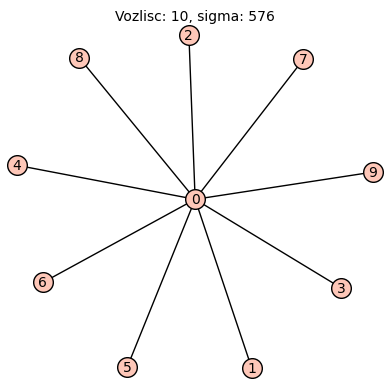
\includegraphics[width=\textwidth]{graf_eno_centralno.png}
      \end{minipage}
      \hfill
      \begin{minipage}[b]{0.32\textwidth}
          \centering
          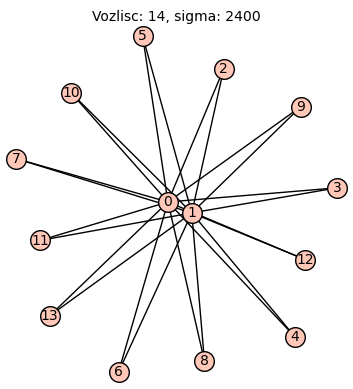
\includegraphics[width=\textwidth]{graf_dve_centralni.png}
      \end{minipage}
      \hfill
      \begin{minipage}[b]{0.32\textwidth}
          \centering
          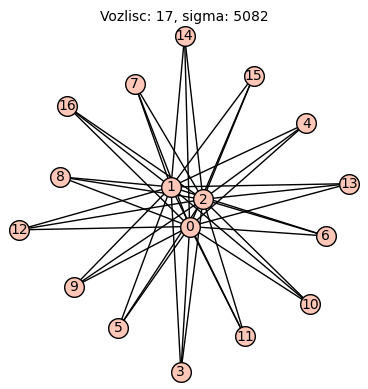
\includegraphics[width=\textwidth]{graf_tri_centralna.png}
      \end{minipage}
  \end{figure}  

Zanimalo naju je tudi, kako narašča število centralnih vozlišč (t.j. število vozlišč v manjši množožici) glede na stopnjo grafa 
in pa kakšno je razmerje med centralnimi in robnimi vozlišči. Opazila sva, da se število centralnih vozlišč enakomerno (skoraj linearno) 
povečuje in ima specifično stopničasto strukturo, skoki pa se pojavljajo na približno enakih razmakih (na približno 7 
do 8 novih vozlišč se doda novo centralno vozlišče). To si lahko razlagamo na način, da dodajanje novih 
vozlišč v graf najprej povečuje število robnih vozlišč, ko dosežemo določen prag, pa se doda še eno centralno vozlišče. 
Izkaže se, da se delež vozlišč v manjši množici dvodelnega grafa z večanjem števila vseh vozlišč giblje med 14\% in 16\%, torej konvergira.
Za boljšo vizualizacijo sva narisala tudi dva grafa.

\begin{figure}[h!]
    \centering
    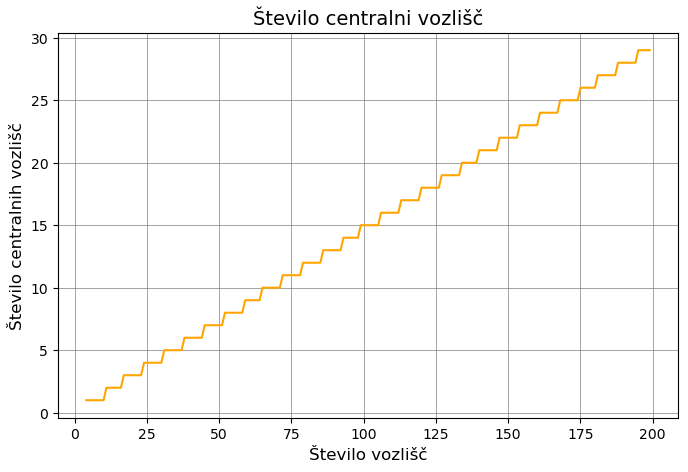
\includegraphics[width=0.85\textwidth]{graf_st_centralnih.png}
\end{figure}

\begin{figure}[h!]
    \centering
    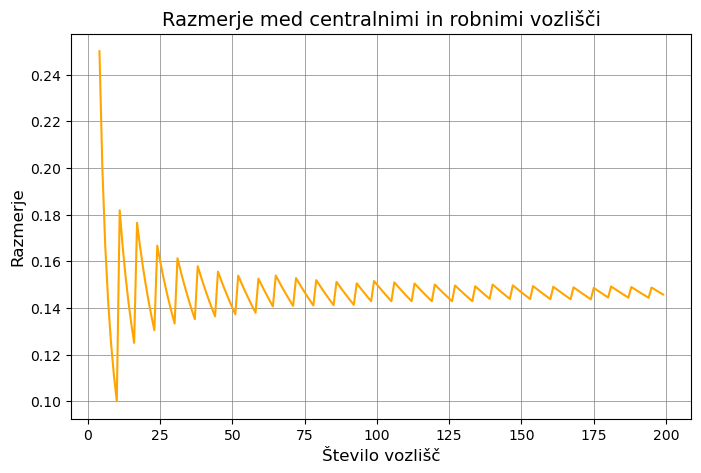
\includegraphics[width=0.85\textwidth]{graf_razmerje_med_centralnimi_in_robnimi.png}
\end{figure}

\section{Testiranje hipotez}
\subsection{Metahevristični algoritmi}
\subsubsection{Simulated annealing}
Osnovna ideja algoritma Simulated annealing je, da v določenih primerih dovoljuje poslabšanja trenutne rešitve, kar omogoča pobeg
iz lokalnih minimumov. Algoritem se začne z generiranjem začetne rešitve (v najinem primeru sva vzela kar zvezdaste grafe z 
največjo možno STI), določimo pa tudi začetno temperaturo. Nato v vsaki iteraciji izberemo novo rešitev in jo sprejmemo glede na 
njeno kakovost v primerjavi s trenutno rešitvijo. Če je nova rešitev, boljša jo sprejmemo, sicer pa jo sprejmemo z določeno 
verjetnostjo (določeno z Boltzmanovo porazdelitvijo).Sčasoma se temperatura zmanjšuje, kar pomeni, da je na začetku verjetnost 
sprejemanja slabših rešitev visoka, nato pa čedalje nižja. Algoritem je enostaven za implementacijo ter zelo prilagodljiv različnim 
optimizacijskim problemom, prednost pa je tudi, da omogoča pobeg iz lokalnih minimumov. Vendar pa je uspešnost močno odvisna od 
začetne temperature in hitrosti ohlajanja, če temperatura upada prehitro ali prepočasi naši rezultati lahko niso točni.

Koda za opisani algoritem je shranjena v datoteki $\texttt{simulated\_annealing.ipynb}$.

\subsubsection{Tabu search}
Tabu Search je metahevristični algoritem za optimizacijske probleme, ki uporablja zgodovino iskanja in omogoča raziskovanje večjega 
iskalnega prostora. Osnovna ideja je uporaba tabu seznama, ki beleži že obiskane rešitve in preprečuje vračanje k njim. Algoritem 
deluje na principu lokalnega iskanja z najboljšo možno izboljšavo, pri čemer se rešitve filtrirajo glede na tabu pogoje – dovoljene 
so samo tiste, ki niso na tabu seznamu, razen če so boljše od trenutne najboljše rešitve. Dolžina tabu seznama (tabu tenure) vpliva 
na širino raziskovanja: krajši seznam omogoča bolj lokalno iskanje, daljši pa raziskovanje širšega prostora. Poleg kratkoročnega spomina 
TS uporablja tudi dolgoročni spomin, ki spremlja pogostost in kakovost rešitev ter usmerja iskanje v manj raziskane ali obetavne regije 
prostora rešitev. Slabost TS je lahko možnost prevelikega izogibanja določenim rešitvam, kar potencialno 
lahko vodi do izgube optimalnih rešitev. 

Koda za opisani algoritem je shranjena v datoteki $\texttt{tabu\_search.ipynb}$.

\subsubsection{Variable neighborhood search}
Algoritem VNS temelji na ideji, da se različne soseščine obnašajo kot različne "pokrajine" iskalnega prostora. Sestavljen je iz treh faz:
\begin{enumerate}
      \item Naključna izbira sosednjega območja (faza perturbacije).
      \item Generiranje novih rešitev v izbrani soseščini, vsakič poskusimo izboljšati rešitev znotraj izbrane soseščine (lokalno iskanje).
      \item Če je nova rešitev boljša od trenutne, jo sprejmemo, sicer ne naredimo ničesar. Znova začnemo iskanje (faza premika).
\end{enumerate}
Prednost VNS je dobro ravnotežje med iskanjem v širino in globino, saj združuje iskanje v lokalnem območju in raziskovanje novih območij. Vendar
pa lahko naletimo do težav, če izberemo napačno soseščino, kar lahko vodi do neučinkovitega iskanja. Poleg tega pa ima algoritem tudi večjo
računsko zahtevnost prav zaradi uporabe več sosedskih struktur.

Koda za opisani algoritem je shranjena v datoteki \\$\texttt{variable\_neighborhood\_search.ipynb}$.

\subsubsection{Mešani algoritem - SA in VNS}
Navsezadnje sva implementirala tudi algoritem, v katerem sva združila simulated annealing in variable neighborhood search (koda se nahaja
v datoteki $\texttt{mix\_SA\_VNS.ipynb}$). Začetek je enak kot pri VNS, torej najprej izberemo sosednje območje in nato izvedemo lokalno iskanje. 
V nadaljevanju pa pri sprejemanju nove rešitve vključimo še SA. Če je nova rešitev boljša od trenutne, jo sprejmemo, slabše rešitve pa sprejmemo
z verjetnostjo, določeno z Botzmanovo porazdelitvijo. 

\section{Ugotovitve}
Z vsemi zgornjimi metahevrističnimi algoritmi sva potrdila najino hipotezo, da imajo polni dvodelni grafi, dobljeni v datoteki 
$\texttt{star\_graphs.ipynb}$, res največje možne STI. Pri implementaciji sva namreč vsakič začela s polnim dvodelnim grafom, ki naj 
bi po najini hipotezi že bil optimalen. Od tam naprej sva sva se z vsakim algoritmom le še bolj oddaljevala od od maksimalne STI, ki
jo je imel izhodiščen graf. 

Ugotovila sva tudi, da razmerje med obema stranema dvodelnega grafa konvergira ko povečujemo stopnjo grafa. Delež vozlišč v manjši 
množici je nekje 14 - 16 \%, delež v večji množici pa 84 - 86 \%. Opazila sva še, da se število centralnih vozlišč (t.j. moč manjše množice 
vozlišč dvodelnega grafa) enakomerno povečuje: za grafe do 10 (t.j. $n = 1, \ldots ,10$) vozlišč imamo 1 centralno vozlišče, nato 2 centralni
vozlišči za $n = 10, \ldots ,16$, novo centralno vozlišče se doda nadaljne še pri $n = 17, n =24, n = 31$ itd.
Skoki se torej pojavljajo na približno enakih razmakih; na vsakih 7 do 8 novih vozlišč se v manjšo množico vozlišč polnega dvodelnega 
grafa doda še eno vozlišče.

\nocite{Luke2013Metaheuristics}

\newpage
\bibliographystyle{plain}
\bibliography{viri_projekt_fp.bib}
      

\end{document}